\section{Stand der Forschung}


Die zunehmende Tendenz in Deutschland von bargeldlose Bezahlung erfordert neuen Umgang mit der 
eigegebenen Daten. Eine Studie von 2009 der Deutschen Bundesbank zeigte die rasante Anstieg von 
bargeldlose Bezahlung in der Bundesrepublik seit der Einführung von solcher Zahlungsmethode 
\cite{refrep:DBCP}.

\begin{figure}[htb]
    \centering{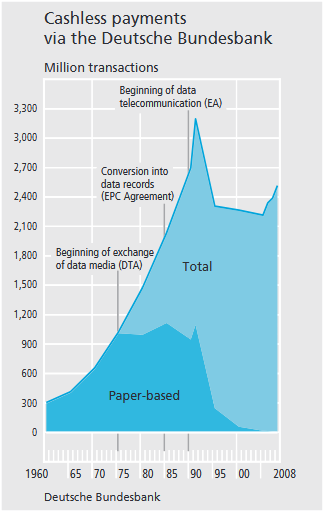
\includegraphics[width=5cm]{Bilder/refrep_DB.png}}
    \caption{Cashless payments via the Deutsche Bundesbank}
    \label{fig:refrep_DB}
\end{figure}


Laut einer Statistik des Handelsforschungsinstituts EHI von 2019 \cite{refart:KSDL} bezahlen 48,6\% 
der deutschen ihre Waren mit Karte, wohingegen nur noch 46,9\% der deutschen den klassischen 
Weg mit Bargeld gehen. Auch das kontaklose Bezahlen, bei dem bei kleinen Beträgen nicht 
einmal eine PIN gefordert wird nimmt immer weiter zu. Doch gerade bei dieser Variante ist es 
sehr einfach im Namen eines anderen zu bezahlen.

\vspace{1cm}

\textbf{Variante 1}
\textcolor{blue}{Immer wenn mit Karte bezahlt wird, geht die Kundinnen davon aus, dass die Zahlungsabwicklung sicher ist.
Wie kann es aber sichergestellt werden, dass bargeldlose Bezahlung sicher heutzutage sicher ist.}


\textbf{Variante 2}  
\textcolor{blue}{Wenn wir heutzutage in einem Supermarkt oder ähnliches mit unserer Karte bezahlen, gehen wir davon
aus, dass die Zahlungsabwicklung sicher ist. Aber sollten wir das einfach so hinnehmen? Wie sicher
ist das bargeldlose Zahlen heutzutage wirklich? \textcolor{red}{Was sagst du über diese Variante 2?}}

\vspace{1cm}



Aus diesem Grund ist Vertraulichkeit das erste und wichtgste Voraussetzung, dass ein solches System 
erfüllt muss, um potenziellen neue Kunden zu gewinnen. Unter diesem Begriff soll ein System nur auf 
autorisierte Informationen zugreifen \cite{refbook:SWIS}. In dieser Hinsicht ist die Entwicklung 
einer Click and Buy Maschine so zu konzipieren, dass sie einen sicheren Umgang mit den Kundendaten
anbietet. Diese Interaktion zwischen Kunde und systemkritischen Mechanismen wurde von \cite{refart:HARE}
so gargestellt: 

\begin{figure}[htb]
    \centering{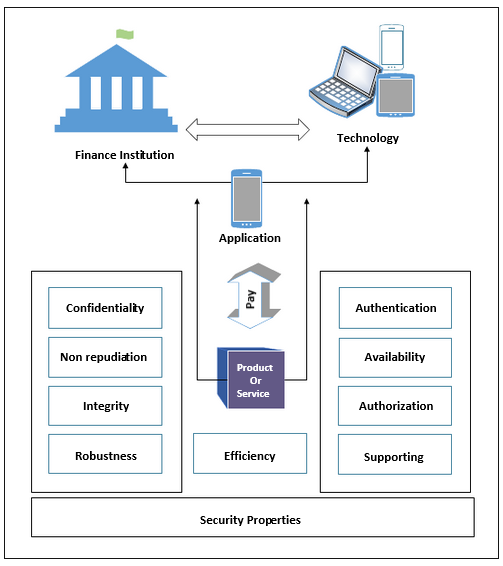
\includegraphics[width=5cm]{Bilder/refark_HARE.png}}
    \caption{Sicherheitseigenschaften von digitalen Zahlungsmethodne}
    \label{fig:refark_HARE}
\end{figure}


Außerdem sollen die anderen Schutzziele der IT-Sicherheit: Integrität, Verfügbarkeit und
Authentifizierung auch berücksichtg werden, so dass die Systemen einwandfrei funktionieren können.
Ein Zahlungsmethode, die alle diese Voraussetzung erfüllt, kann in der Lage sein, das Vertrauen und 
die Akzetanz von Nutzenden zu bekommen \cite{refart:HARE}. \par


\cite{inbook:MHNS} nennt solche Maschinen Cyber-Physical System (CPS), weil sie eine Interaktion zwischen 
Nutzer und ein oder mehrere Systemen darstellt. In dieser Zusammenarbeit spielt den Datenaustausch 
eine wesentliche Rolle, besonders von der Seite der Nutzender. Diese Technologie zielt eine günstigere 
Entwicklung, ohne auf die Sicherheit zu vernachlässigen. Diese Interaktion findet erfolgereich statt, 
wenn die genannten Sicherheitszielle erfüllt werden.


Da es sich um einen dynamischen Sektor geht, finden die Änderungen sehr schnell statt, obwohl die 
Sicherheitsmechanismen an diese Geschwindigkeit nicht immer anpassen können \cite{refbook:MNIT}.
Das kann schlimme Folge für die Weiternutzung solcher Technologie. 


\textcolor{red}{Ab hier können wir dann versuchen, die Informatien aus den Artikeln zu nehmen, solche
die du hier hinzugefügt hast und solche, die ich dir am Fr schickte}










\textbf{Ich würde diesen Satz in den nächsten Kapitel verwenden und erweitern mit unseren Recherchen, damit wird 
die Literatur rechtfertigen können}
Um das zu bewerkstelligen, ist der aktuelle technische Stand von entscheidener Bedeutung. 
Ausgehend von dieser Informationen muss das Glasfasernetz eventuell erweitert oder auch neu verlegt werden.
Denn das Ziel ist es, technisch gesehen auf dem neusten Stand zu sein, damit das Click and Buy System für die Zukunft abgesichert ist.
Außerdem wird durch den Ausbau des Glasfasernetzes die Region insgesamt deutlich attraktiver gemacht, was vielleicht auch Menschen dazu bringt
in diese Region zu ziehen. Denn jedem ist klar, dass ein guter Internetausbau essentiell ist, um vielleicht auch mal von zuhause aus zu arbeiten.













